\chapter{General Equilibrium}
While we've done a lot of economics so far, we have not actually modeled a full economy yet! We've instead focused on studying what is known as \vocab{partial equilibrium}, which examines how agents optimize their behavior taking the other side of the market. For example, when we study the firm optimization problem, we take the price of the good as given and assume there are some consumers who are willing to buy the goods at that price. Similarly, when we studied consumer theory, we assumed that consumers could always buy goods at a given price, and we do not model how the firms actually produce those goods. In both cases, we did not concern ourselves with how prices or wages are set. However, in real economies, prices depend on how agents in the economy behave and the decisions that they make. In this section, we will model a \vocab{general equilibrium}, which considers how individual optimizations leads supply and demand in markets clearing through appropriately set prices. In a general equilibrium model, rather than prices being exogenous, they will be endogenously determined by supply and demand, and the only truly exogenous variables will be the so-called economic ``primitives,'' which are coefficients that determine an individual's utility function, productivity, etc., and we will have truly modeled a full economy. 

\section{Exchange Economy}
We will start by considering a very simple economy in general equilibrium: an \vocab{exchange economy}. In an exchange economy, agents have initial endowments of goods that they can buy and sell from each other. Rather than agents producing goods, we assume that agents are just exchanging existing goods. While this might seem very different from the economies that we've examined so far or even the economies that you are familiar with. However, the exchange economy allows us to examine the fundamental role of prices, and why markets can make everyone better off regardless of what endowments the agents start with.

\subsection*{Setup}
An exchange economy has multiple components, some of which will differ from the standard models that we have examined so far. We establish what these components are here.

\begin{description}
    \item[Agents] In contrast to partial equilibrium models where we can examine the economy from the perspective of a single agent, because there is trading in the exchange economy, we need to quantify the number of agents. For simplicity, we will assume that there are $N$ agents.\footnote{
        Note that we are implicitly assuming here that there are a finite number of agents. However, we could also treat this assumption as there being $N$ \emph{types} of agents, where agents of the same type behave identitically, and there is a continuum of agents of each type. This allows us to more reasonably treat the agents as price-takers, as there may be an infinite number of agents of each type. 
    } We can ``name'' these agents from $1, \dots, N$. When we are describing some property $x$ that applies to a given agent, we will use superscripts, and the index $i$, so $u^i$ might denote the utility function for the $i$th agent. 
    \item[Goods] We assume that there are $M$ different goods, and we name these goods $j = 1, \dots, M$. We will use subscripts to describe variables relating to a particular good. So $x^i_j$ might denote the demand for good $j$ by agent $i$. 
    \item[Endowments] We assume that agents have some exogenous amount of each good to start with. Agent $i$ has $w^i_j$ units of good $j$. In vector notation, we can describe agent $i$'s endowment as $\vec{w}^i \in \R^M$. 
    \item[Utility functions] We assume that each agent has a utility function, $u^i(\cdot)$ and that the arguments to the utility function are the goods that the agent receives, and \emph{only} the goods that the agent receives. While this might seem like a simple assumption on the utility function, it rules out cases like externalities where an agent's utility depends on how much another agent consumes of a particular good. 
    \item[Prices] We assume that every agent faces the same price $p_j$ for good $j$. This means that we can describe the prices in the economy as a whole by $\vec{p} \in \R^M$. Importantly, we assume that each agent is a \emph{price-taker}, meaning that the agent does not assume that their choices are able to affect the global prices. This is of course not in general true, in cases like monopoly or monopsony, but it is a reasonable assumption for cases where $N$ is large.     
\end{description}

\subsection*{Walrasian Equilibrium}
Now that we have established the basic setup of the economy, we will describe what it means for the economy to be in equilibrium. A general equilibrium of the economy satisfies the following: 
\begin{description}
    \item[Individual optimization] Each agent $i$ chooses consumption $x_j$ of good $j$ to optimize their utility function, $u^i(\vec{x})$ subject to the following constraint,
    \begin{equation} \label{eq:ge_budget_constraint}
        \sum_{j = 1}^M p_j x_j \leq \sum_{j = 1}^M p_j w^i_j 
    \end{equation} 
    This says that the market value of our total consumption can be at most the market value of our initial endowment of goods. In essence, we are treating the market value of our initial endowment as our income. Written in vector form, agent $i$ solves the maximization problem,
    \begin{align*}
        \vec{x}^i = \argmax_{\vec{x}}u^i(\vec{x}) \text{ s.t. } \vec{p} \cdot \vec{x} \leq \vec{p} \cdot \vec{w}^i
    \end{align*}
    $\vec{x}^i(\vec{p})$ is the agent's Marshallian demand function for each of the goods, and notice that it will be a function of the prices. Each individual agent treats these prices as given, and solves the optimization assuming that their demand will have no effect on the price. 

    \item[All markets clear] The price vector, $\vec{p}$ is set to ensure that the total demand for each good is equal to the total endowments of each good. This is known as \vocab{market clearing}. That is, $\vec{p}$ must be such that for every good $j$, 
    \begin{align*}
        \sum_{i = 1}^N x^i_j(\vec{p}) = \sum_{i = 1}^N w^i_j(\vec{p})
    \end{align*}  
    Or more succinctly in vector notation,
    \begin{align*}
        \sum_{i = 1}^N \vec{x}^i(\vec{p}) = \sum_{i = 1}^N \vec{w}^i(\vec{p})
    \end{align*}
    Another formulation of this condition is to consider the \vocab{excess demand function} for a particular good, which is the difference between the total demand of a good and the total supply of that good. In an exchange economy, the total supply of a good is simply the total endowments of that good. So, the excess of demand function of good $j$ with prices $\vec{p}$ is given by
    \begin{align*}
        f_j(\vec{p}) = \sum_{i = 1}^N x^i_j - w^i_j
    \end{align*}
    In an equilibrium, we need prices $\vec{p}^*$ such that,
    \begin{align*}
        f_j(\vec{p}^*) = 0 \; \text{for all $j$}
    \end{align*}
    That is, a given market clears if that market has no excess demand.\footnote{
        Excess demand functions are of special importance in the study of general equilibria. While we will not consider the stability of general equilibria in this course, it is often assumed that a reasonable price adjustment process for a particular good $j$ is an increasing function of $f_j(\vec{p})$. That is, the market prices converge to equilibrium by adjusting upwards when there is too much demand in a particular market, and adjusting downwards when there is too little demand. If such a price adjustment process converges to an equilibrium, that equilibrium is called stable. It is known that even under very reasonable assumptions and a basic economy, general equilibria can fail to be stable. 
    }
\end{description}
A set of demand functions $\{\vec{x}^i\}$ and prices $\vec{p}$ that satisfy the above is known as a \vocab{Walrasian equilibrium}, which is the type of general equilibrium that we will focus on in this course. Later in this chapter, we will cover the basic properties of a Walrasian equilibrium, and whether they are guaranteed to exist. 

\subsection*{Walrasian Auctioneer}
We have required that in equilibrium, the prices, $\vec{p}$ are such that every market clears. However, we do not specify how the prices actually get to an equilibrium. The process of prices converging to an equilibrium is known as \emph{tâtonnement}, which is French for ``trial and error.'' However, the \emph{tâtonnement} process is not yet well understood, and it has been shown that under some very reasonable assumptions on preferences and adjustment processes that prices will not converge to a stable equilibrium.

Instead, eeconomists usually imagine the market matching mechanism as taking place through a \vocab{Walrasian auctioneer}, who takes in the demand functions from each agent, and selects the prices that will ensure the market clears. It is important to note however that this is simply a description of how one might reach a Walrasian equilibrium, and that economists do not actually think such an auctioneer exists. Nonetheless, the idea of a Walrasian auctioneer may be a reasonable approximation for how we would expect prices to behave in competitive markets.

\subsection*{Extending to Production Economies}
The model we have developed so far considers only exchange economies where agents have some exogenous endowment of goods that can be traded. It is relatively easy to extend this to economies where agents are producing new goods. After all, the basic principles are the same: there is a supply and demand for goods, and the price is that which makes sure the market clears. However, we simply introduce a new type of agent: the firm, which does not have an initial endowment, and instead chooses how much labor to hire and how much capital to purchase. We set up a very simple model of each below.

\begin{description}
    \item[Firms] Suppose we have $M$ identitical firms with production function $f(L)$ that is strictly increasing and concave, as usual. The firm chooses how much labor to hire at some wage $w$, and can sell their goods for a price $p$. The firm's optimization problem is therefore,
    \begin{align*}
        \max_{L} p f(L) - wL
    \end{align*}  
    Let $L_{f}^*(p, w)$ be the firm's optimal choice of labor
    \item[Consumers] Suppose we have $N$ consumers who have preferences over consumption and labor. The worker's utility function is therefore $U(C, L)$. The workers both consume the firms goods, and supply the firms labor. The agents face price $p$ per unit of consumption, and wage $w$ for each unit of labor. Suppose each agent has exogenous income $y$. The agent's maximization problem is therefore:
    \begin{align*}
        \max_{C, L} u(C, L) \text{ s.t. } pC = wL + y
    \end{align*} 
    Let $C^*(p, w), L_{c}^*(p, w)$ be the consumer's optimal choice of consumption and labor, respectively. 
    \item[Clearing markets] There are two markets that we need to clear here: the market for goods and the market for labor. The market for labor is straightfoward. We have a labor supply from the workers, and labor demand for the firms. We have $M$ firms and $N$ workers so, 
    \begin{align*}
        M L_{f}^*(p, w) = N L_{c}^*(p, w)
    \end{align*} 
    We also require that the firms produce as much as the consumers buy. So we need,,
    \begin{align*}
        M f(L^*(p, w)) = N C^*(p, w)
    \end{align*}
    Notice that we know have two equations and two remaining endogenous variables, $p$ and $w$, from the point of view of the model, which means that we can solve for them.
    \item[Normalizing prices] One thing you may notice, however, is that if you were to actually solve for $p$ and $w$ in a general way, you would only be able to determine the ratio, $\frac{p}{w}$. The reason is because money is just some unit of measurement. We could measure in dollars, pennies, or euros, and the distribution of goods in the real economy should not change. As a result, it is standard to \emph{normalize} one of the prices to $1$. In the next section, we will offer a theorem on why this is possible. 
    \item[Where do profits go?] One question that arises from a production economy of general equilibrium is where the firm's excess profits go. Right now we do not account for the profits, and so our economy is essentially ``losing'' money, which does not occur in the real economy when firms make profits. The typical assumption is that firm profits are rebated to workers (you can think of the workers are shareholders), but that the workers do not internalize their effect on profits when making their labor or consumption choices. While we will not make this addition here, it is a fairly simple extension of the model that can be applied in your own models of production in general equilibrium.  
\end{description}

\section{Properties of Walrasian Equilibrium}
In this section, we will discuss some of the key properties and theorems related to Walrasian Equilibria.

\subsection*{Existence}
One of the main questions is whether a Walrasian equilibrium exists at all. Is it true for every set of initial endowments and every set of utility functions that a price vector will exist to clear the markets? The answer is non-obvious, but fortunately, there do exists very weak assumptions on the agent's utility functions that guarantee the existence of a Walrasian Equilibrium. To do so, we need to first define \vocab{convex preferences}.

\begin{definition*}[Convex preferences]
    A preference relation $\precsim$ is convex if for any bundles of goods, $\vec{x}, \vec{y}, \vec{z}$ where $\vec{x} \succsim \vec{z} $ and $\vec{y} \succsim \vec{z}$, then for any $\lambda \in [0, 1]$,
    \begin{align*}
        \lambda \vec{x} + (1 - \lambda) \vec{y} \succsim \vec{z}
    \end{align*}
    In utility function form, we have,
    \begin{align*}
        u(\vec{x}) \geq u(\vec{z}), u(\vec{y}) \geq u(\vec{z}) \implies u(\lambda \vec{x} + (1 - \lambda)\vec{y}) \geq u(\vec{z})
    \end{align*}
\end{definition*}

Now, we can offer the following existence theorem, which we will not prove because the proof is beyond the scope of this course,
\begin{theorem*}[Existence of Walrasian Equilibrium]
    In an exchange economy where agents have convex preferences, every good is desirable, and the consumption of a good only affects the utility of the agent consuming it, there exists a Walrasian equilibrium. 
\end{theorem*}
By every good being desirable, we mean that for every agent, their utility must strictly increase if they consume more of a particular good. While the assumptions on this theorem are relatively weak, they do rule out some key cases, such as goods where consuming one good has an externality effect on the other agents.

While the above existence applies to exchange economies, there is one additional requirement for the existence of a general equilibrium in a production economy: the production function must be concave. This rules out cases of increasing returns to scale. 

\subsection*{Walras's Law}
When solving for a general equilibrium model with $M$ goods, we usually are only able to solve for the ratio of the equilibrium prices between those goods, so we will typically normalize the price of one of the goods to $1$. The economic intuition here is that of monetary neutrality: it does not matter what units we measure prices in, but only that they are consistent relative to each other. 

However, we want to make sure that even if we normalize the price of a given item to $1$, that the market still clears. To do so, we use a result known as Walras's Law:

\begin{theorem*}[Walras's Law]
    In an economy where agents face budget constraints, the sum of the values of the excess demands in all markets must be zero, regardless of prices. More formally, let $\vec{p}$ be an arbitrary price vector with $N$ individuals and $M$ goods. Let $\vec{x}^i$ denote the Marshallian demand function and let $\vec{w}^i$ be the endowment vector for each agent $i$. Then,
    \begin{align*}
        \sum_{i = 1}^N \vec{p} \cdot (\vec{x}^i - \vec{w}^i) = 0
    \end{align*}
\end{theorem*}
\begin{proof}
    The proof of Walras's Law is fairly straightfoward if we know that budget constraints are satisfied. By the definition of the budget constraint of agent $i$, we know that
    \begin{align*}
        \vec{p} \cdot \vec{x}^i = \vec{p} \cdot \vec{w}^i \iff  \vec{p} \cdot \vec{x}^i - \vec{p} \cdot \vec{w}^i = 0 
    \end{align*}
    Hence, the total value of excess demand in the economy is,
    \begin{align*}
        \sum_{i = 1}^N \vec{p} \cdot (\vec{x}^i - \vec{w}^i) &= \sum_{i = 1}^N  (\vec{p} \cdot \vec{x}^i - \vec{p} \cdot \vec{w}^i) \\
        &= \sum_{i = 1}^N 0 \text{ by the budget constraint}\\
        &= 0 
    \end{align*}
\end{proof}

Walras's Law offers an important corollary that allows us to normalize prices:
\begin{corollary*}
    If an economy with $n$ goods and positive prices has markets clear in $n - 1$ of those goods, then the $n$th market must also clear.
\end{corollary*}

\begin{proof}
    Let $z_j$ be the total excess demand for good $j$. Suppose without loss of generality that $z_j = 0$ for $j = 1, \dots, n - 1$. That is, the market clears for $n - 1$ goods. Let $\vec{p}$ be the the corresponding price vector. By Walras's law, we know that, 
    \begin{align*}
        \sum_{j = 1}^n p_j z_j = p_n z_n = 0
    \end{align*}
    Because by assumption, $p_j z_j = 0$ for all $j < n$. Since $p_n > 0$ by assumption of positive prices, we conclude that $z_n = 0$. That is, the excess demand in the $n$th market is 0, which means that the market clears. 
\end{proof}
For us, this means that if we normalize the price of a given good to $1$, and we adjust prices to clear in all the other markets, then the market for that good must also clear. 

\subsection*{Pareto Efficiency}
Before covering two welfare theorems associated with Walrasian equilibria, we will consider one way of defining whether an economy is peforming ``optimally.'' The concept of Pareto efficiency is widely used in microeconomic theory, and offers a very weak condition for the optimality of an economy.

\begin{definition*}
    An allocation is \vocab{Pareto efficient} if, in order to strictly improve the welfare of one agent, the welfare of another agent must strictly decrease. 
\end{definition*}
In some sense, Pareto efficiency is the most basic property you would want an optimal outcome to have. If there existed an alternative allocation of goods where you could make a given agent better off without making any agents worse off, most would agree that by any reasonable standard, that alternative allocation is preferable. 

However, it is important to note that Pareto efficiency is a very weak condition. For example, an allocation where all of the goods in the economy go to one individual is Pareto efficient. However, to get stronger conditions of optimality for an allocation of goods, you may need to bring in interpersonal comparisons of utility, which economists try to avoid. 

\subsection*{First Welfare Theorem}
The First Welfare Theorem tells us a key property about the efficiency of Walrasian equilibria:

\begin{theorem*}[First Welfare Theorem]
    Every Walrasian equilibrium is Pareto efficient. 
\end{theorem*}
\begin{proof}
    Let $\vec{w}^i$ be the endowents and let $u^i$ be the utility function for agent $i$. A Walrasian equilibrium is characterized by prices $\vec{p}$ and allocations $\{\vec{x}^i\}_{i = 1}^N$. Suppose we have some alternative allocation $\{\vec{z}^i\}_{i = 1}^N$ where at least one agent is strictly better off. Let $i^*$ be such an agent: 
    \begin{align*}
        u^i(\vec{z}^{i^*}) > u^i(\vec{x}^{i^*})
    \end{align*}
    However, since, in the Walrasian equilibrium, $i^*$ is optimizing, then $\vec{z}^{i^*}$ must not be affordable at prices $\vec{p}$, because if it were, then the agent would have already purchased $\vec{z}^{i^*}$. So,
    \begin{align*}
        \vec{p} \cdot \vec{z}^{i^*} > \vec{p} \cdot \vec{x}^{i^*}
    \end{align*}
    If we assume that no other individual is strictly worse off, then for every agent $i$, we must have that
    \begin{align*}
        u^i(\vec{z}^i) \geq u^i(\vec{x}^i) \implies \vec{p} \cdot \vec{z}^i \geq \vec{p} \cdot \vec{x}^i
    \end{align*}
    Where the inequality is strict for $i^*$. Summing over all agents therefore yields,
    \begin{align*}
        \sum_{i = 1}^N \vec{p} \cdot \vec{z}^i = \vec{p} \cdot \sum_{i = 1}^N \vec{z}^i > \vec{p} \cdot \sum_{i = 1}^N \vec{x}^i = \sum_{i = 1}^N \vec{p} \cdot \vec{x}^i
    \end{align*}
    However, recall in both cases, we require the total allocations to be equal to the total initial endowments, so we have,
    \begin{align*}
        \sum_{i = 1}^N \vec{z}^i = \sum_{i = 1}^N \vec{w}^i = \sum_{i = 1}^N \vec{x}^i
    \end{align*}
    Substituting into the above inequality then yields,
    \begin{align*}
        \vec{p} \cdot \sum_{i = 1}^N \vec{w}^i > \vec{p} \cdot \sum_{i = 1}^N \vec{w}^i
    \end{align*}
    This is a contradiction, and hence we know that in a Walrasian equilibrium, no agent can be made better off without making at least one other agent worse off. So, the resulting allocation must be pareto efficient. 
\end{proof}

The First Welfare Theorem tells us that, at least in a very basic sense, competitive equilibria are efficient because no person can be made better off without making another first off. In other words, there are no ``welfare arbitrage'' opportunities where a social planner could intervene and make everyone better off. The economic intuition here is that if two agents could be made better off without making either worse off, they could trade with each other, and the equilibrium sets the prices so that everyone who is willing to trade with each other does so. 

\subsection*{Second Welfare Theorem}
While the First Welfare Theorem told us that every Walrasian Equilbirium is Pareto efficient, the Second Welfare Theorem tells us the converse: that every Pareto efficient outcome can be the result of a Walrasian equilibrium with appropriate prices and initial endowments. 

\begin{theorem*}[Second Welfare Theorem]
    Any Pareto efficient allocation $\{\vec{x}^i\}$ forms a Walrasian equilibrium with some prices $\vec{p}^i$ and some initial endowments, $\vec{w}^i$.
\end{theorem*}
\begin{proof}
    Let $\{\vec{x}^i\}$ be a Pareto efficient allocation. Our goal is to construct some initial endowments $\{\vec{w}^i\}$ such that the resulting equilibrium prices $\vec{p}$ yield the allocation $\{\vec{x}^i\}$. The intuitive guess is to set $\vec{w}^i = \vec{x}^i$ for all agents $i$. That is, we are simply setting the initial endowments to be equal to the desired final allocation. Let $\vec{p}$ be the vector of prices and let $\{\vec{z}^i\}$ be the allocation resulting from the Walrasian equilibrum with our constructed endowment. We will assume that preferences are such that the Walrasian equilibrium exists.

    We need to show that every agent weakly prefers $\vec{x}^i$ to $\vec{z}^i$, $u^i(\vec{x}^i) \geq u^i(\vec{z}^i)$ for all agents $i$. We know that every agent could afford to keep their current bundle, $\vec{x}^i$, and we know that $\{\vec{x}^i\}$ is a Pareto efficient allocation (by assumption). This means that if there were some agent $i^*$ who strictly preferred $\vec{z}^{i^*}$ to $\vec{x}^{i^*}$, then some other agent $j^*$ must be made worse off and strictly prefer $\vec{x}^{j^*}$ to $\vec{z}^{j^*}$. But this means that the agent is not optimizing, because the agent could afford $\vec{x}^{j^*}$, a contradiction. 

    Hence, every agent must weakly prefer $\vec{x}^i$ to $\vec{z}^i$, which means that $\{\vec{x}^i\}$ is an equilibrium allocation with initial endowments $\{\vec{w}^i\}$
\end{proof}
The intuition for the Second Welfare Theorem is that if there was some Pareto efficient allocation in an economy that we wanted to obtain, we could just start off by giving everyone that allocation. Even if people were allowed to trade, they would keep their initial endowments because anything else would necessarily make them worse off in a competitive market.

This has particular importance in economic policy, because it tells us that if we can make lump sum transfers between agents, then if there is some Pareto efficient allocation you want to achieve, you can just use lump sum taxes and subsidies to achieve that allocation.

\section{Recap of GE}
For the first time in this course, we have learned how we can fully model an economy, and we finally know how those exogenous prices might be determined in the real world. We will quickly recap some of the key steps in how to solve for a general equilibrium, as well as the limitations facing Walrasian equilibria in particular.

\subsection*{Solving for Walrasian Equilibrium}
While Walrasian equilbria might seem complicated at first, but can in fact be boiled down to three simple steps. 
\begin{enumerate}
    \item Set up each agent's maximization problem taking prices as exogneous. Solve for their optimal choices in the same way that we would in a partial equilibrium. The supply/demand functions should only depend on prices and other exogenous variables. 
    \item Taking each agent's behavior under particular prices as given, set the supply and demand in each market to be equal. This is the same as setting the excess demand in each market to 0. Normalize one of the prices to $1$. Then, solve for the remaining prices via your system of equations. The prices should only depend on exogenous variables.
    \item Plug in the prices that you calculated from step 2 back into optimal choices that you computed in part 1. This will tell you the final allocations for each agent, and it should only depend on exogenous variables. Prices should not appear in your final allocations.
\end{enumerate}

\subsection*{Limitations of Walrasian Equilibria}
Finally, while Walrasian equilibria are a foundational component of microeconomic theory, there are some important limitations to keep in mind.
\begin{description}
    \item[No externalities] When modeling Walrasian equilibria, we assume that one agent's consumption cannot affect another agent's consumption. This explicitly rules out both positive and negative externalities.
    \item[Non-satiation] We assume that each agent prefers more of a good than less of it, and that no good can make an agent worse off by having more of it. This is often not the case in the real world, and may make modeling a market for, say pollution, much more difficult.
    \item[Perfect information and markets] While this assumption is implicit via the ``Walrasian auctioneer,'' we assume that agents have perfect information about each other's utility functions and prices, and that there are no costs to transactions. This is often not the case in the real world, as most transactions involve one party having more information than the other, and many transactions involve costs beyond price, like travel or negotiation costs. Embedded in this assumption is that agents cannot lie about their demand to try to manipulate the market price to be lower. Each agent reports demand as if their behavior will not change the price.  
\end{description}
In the following chapters, we will relax some of these assumptions and examine the role of government policy in correcting imperfect markets, as well as how agents may behave differently in cases of imperfect information or where agents know they can affect the price. 


\section{Social Conflict in General Equilibrium*}
Most economic models assume that property rights are secure. However, this is often not the case. Property rights are threatened by individual criminals, gangs, and also extractive governments. \citet{dalbodalbo} points out that insecure property rights can cause distortions in the economy and make some seemingly unambiguously good things (e.g., A rise in productivity) have adverse consequences. This model is quite different from the other models in our class because we don't explicitly model for agents optimizing. Instead, the model classifies what the general equilibrium of the economy would look like subject to no-arbitrage conditions (i.e., nobody could do something else and get a better outcome).

\citet{dalbodalbo} writes down a model of an economy with an appropriations sector in equilibrium. They are most interested in how this equilibrium shifts in response to various shocks to the system. To give a real-world example: what do we expect to happen to civil war in Columbia when the price of coffee---a labor-intensive good---increases \citep{dube2013commodity}? Our model not only gives us the potential sign of the change but also tells us why this change occurred.
\subsection*{Setup}
We start with a three-sector economy. Sectors one are two are productive sectors that produce output $q_1$ and $q_2$ using labor ($L$) and capital ($K$) according to some constant returns to scale function. The price of labor is $w$ and the rental price of capital is $r$. There is a total stock of $\bar{L}$ labor and $\bar{K}$ capital (i.e., fixed factor endowments). Sector $A$ is an appropriation sector that uses only labor ($L_A$) and steals a proportion of total output according to some appropriations function $A(L_A)$, where $A(0) \geq 0$, $A(\bar{L}) \leq 1$, $A'(L_A) > 0$ and $A''(L_A) < 0$. The price of $q_1$ and $q_2$ are \emph{exogenously given}. This is very important to understand: we do not get to pick these prices! Unlike the canonical general equilibrium model you've just seen, we are not solving for prices but taking prices as a parameter. The intuition is that we are modeling some export economy where prices are set by the international market. We normalize the price of good two to be one and the price of good one as $p_1$.

The amount stolen from the two productive industries is thus $A(L_A)(p_1q_1 + q_2)$, or $A(L_A)[w(\bar{L} - L_a) + r\bar{K}]$---in a single-period closed economy without investment, all wages/investment returns are consumed.

Workers decide between entering the productive industry and receive wage $[1 - A(L_A)]w$ or joining the criminal industry and receive wage $\frac{A(L_A)}{L_A}[w(\bar{L} - L_a) + r\bar{K}]$
\subsection*{Equilibrium}
Throughout this section, we will focus on equilibriums without specialization (i.e., $q_1 > 0 < q_2$). We define $a_{ij}$ as the minimum amount of factor $j$ needed to produce output in industry $i$ at the minimum cost given $r$ and $w$. That is, $a_{ij}$ will be a function of $r$ and $w$, but we omit it in the notation.\footnote{I will admit that I am personally not very comfortable with this notation. It seemed to come from papers like \citet{Jones1965GE} if you want to dig deeper. If it makes you more comfortable, we could also assume a Leontief production function (i.e., $y_i = \min\{a_{iL}L, a_{iK}K\}$) for our market, and the meaning of $a_{ij}$ becomes apparent. } 

Three sets of conditions capture the general equilibrium of our economy, which is a set of factor prices $w$ and $r$ (once again, $p_1$ is set exogenously), a set of quantities to produce in each sector $q_1$ and $q_2$, and factor use in each sector $(K_1,K_2,L_1,L_2,L_A)$. First, our firms make zero profits:
\begin{equation}\label{eq:p_1rw}
    ra_{1K} + wa_{1L} = p_1
\end{equation}
\begin{equation}\label{eq:rw2}
    ra_{2K} + wa_{2L} = 1
\end{equation}
Secondly, factor markets must clear (i.e., we use up all of our labor and capital)
\begin{equation}\label{eq:Kclear}
    q_1 a_{1K} + q_2 a_{2K} = \bar{K}
\end{equation}
\begin{equation}\label{eq:Lclear}
    q_1 a_{1L} + q_2 a_{2L} =\bar{L} - L_A
\end{equation}
Finally, we have this no-arbitrage condition where labor must earn the same in the productive and appropriation industries. The argument here is that if the two differ, then labor will move from one to the other until they balance out.
\begin{equation}\label{noabitrage}
    \frac{A(L_A)}{L_A}[w(\bar{L} - L_A) + r\bar{K}] = [1 - A(L_A)]w
\end{equation}

The first set of equations helps us set wages and rent, the last one determines $L_A$, and the second set gives us the quantity. From there, we can use the production technologies to back out the amount of labor and capital used in each sector. However, we are primarily interested in the size of the appropriations sector and the economy in general.

The factor prices $r$ and $w$ are completely determined based on the first two equations. Note that these are the gross prices, not the actual take-home profits, which need to be multiplied by $(1 - A(L_A))$ to account for appropriation. We can rewrite equation \ref{noabitrage} as $A(L_A) = \frac{wL_A}{w\bar{L} + r\bar{K}}$. Thus, if $A(0) = 0$ and $A'(0) >\frac{w}{w\bar{L} + r\bar{K}}$, then the concavity of the appropriations technology function implies that there is a unique equilibrium with positive amounts of appropriation. If $A(0) > 0$ (perhaps some production is lost regardless of labor participation in appropriations), then the equilibrium is unique.

\begin{figure}[H]\label{fg:equi}
    \centering
    \caption{The x-axis here is $L_A$, and the appropriation function is $A(L_A)= \sqrt{L_A}$}
    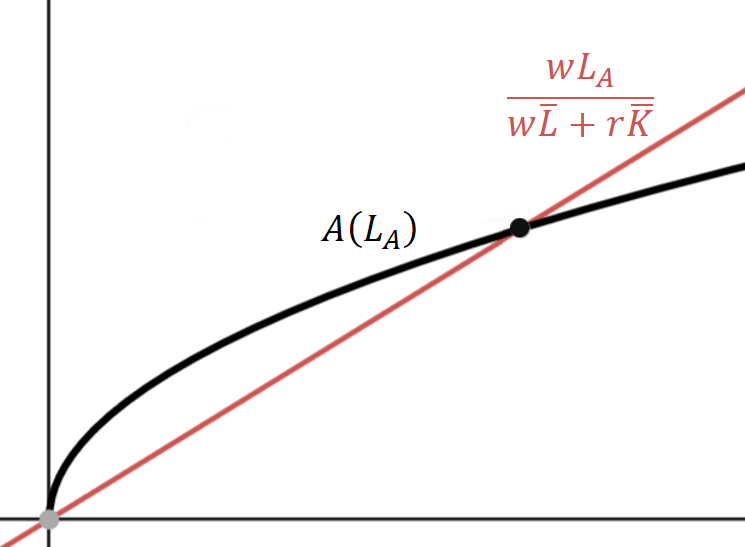
\includegraphics[width = 3.5in]{chapters/Conflict Equilibrium.png}
\end{figure}

\begin{proposition}
    If there exists an equilibrium without specialization when appropriation is not possible, then there exists an equilibrium with some positive amount of conflict and $L_A$ without specialization if $A'(0)$ is sufficiently large and $A(\bar{L})$ is sufficiently small.
\end{proposition}
\begin{proof}
    First, we note that the condition for no specialization in a world without appropriation is $\frac{a_{2K}}{a_{2L}} < \frac{\bar{K}}{\bar{L}} < \frac{a_{1K}}{a_{1L}}$. If there is appropriation, the condition becomes $\frac{a_{2K}}{a_{2L}} < \frac{\bar{K}}{\bar{L} - L_A} < \frac{a_{1K}}{a_{1L}}$. 

    Thus, in order for there to be an economy without specialization and positive amounts of appropriation, the $L_A^*$ that solves equation \ref{noabitrage} needs to be sufficiently small.
\end{proof}
\subsection*{Results}
As a general equilibrium model, however, the $L_A^*$ that solves the no-arbitrage condition (equation \ref{noabitrage}) goes back into the model and tells us about the conditions in the goods market, specifically:
\begin{proposition}
    The appropriations sector increases the production of the capital-intensive good compared to the labor-intensive good.
\end{proposition}
\begin{proof}
    Rearranging equations \ref{eq:Kclear} and \ref{eq:Lclear} yields
    \begin{align*}
        q_1 & = \frac{a_{2L}\bar{K} - a_{2K}(\bar{L} - L_A)}{a_{1K}a_{2L} - a_{1L}a_{2K}} \\ 
        q_2 & = \frac{a_{1K}(\bar{L} - L_A) - a_{1L}\bar{K}}{a_{1K}a_{2L} - a_{1L}a_{2K}}
    \end{align*}
    Since all of the $a_{ij}$'s are positive, it's clear that an increase in $L_A$ will increase the numerator of $q_1$ and decrease the numerator of $q_2$. Thus for $\pd{q_1}{L_A} > 0$, we need to show that the denominator is positive, which follows from the assumption that $\frac{a_{2K}}{a_{2L}} < \frac{a_{1K}}{a_{1L}}$.
\end{proof}

\begin{lemma}
An increase in the price of the capital-intensive good ($p_1$) will decrease wages and increase rents.
\end{lemma}
\begin{proof}
    Differentiate equations \ref{eq:p_1rw} and \ref{eq:rw2} with respect to $p_1$ on both sides and applying envelope theorem (i.e., $\pd{a_{ij}}{p_1} = 0$ for all $ij$) gives us a system of linear equations. Applying some linear algebra gets us
    \begin{align*}
        \frac{dw}{dp_1} & = \frac{-a_{2K}}{a_{1L}a_{2K}-a_{2L}a_{1K}} < 0 \\ 
        \frac{dr}{dp_1} & = \frac{a_{2L}}{a_{1L}a_{2K}-a_{2L}a_{1K}} > 0
    \end{align*}
\end{proof}
The two key results of the paper are the following:
\begin{proposition}
    An increase in the price of the capital-intensive good results in the expansion of the appropriations sector.
\end{proposition}
\begin{proof}
    Starting with $A(L_A) = \frac{L_A}{\bar{L} + r/w\bar{K}}$, we write $L_A$ as a function of $p_1$ and differentiate. Rearranging gets us
    $$\frac{dL_A}{dp_1} = - \left[A' - \frac{1}{\bar{L} + r/w\bar{K}}\right]^{-1}\left[\frac{KL_A}{(\bar{L} + r/w\bar{K})^2}\frac{d(r/w)}{dp_1}\right]$$
    From the previous lemma, we know that $\frac{d(r/w)}{dp_1}$ is positive. Thus, in order for $\frac{dL_A}{dp_1} > 0$, the only assumption we need is $A'(L_A) < \frac{1}{\bar{L} + r/w\bar{K}}$. This result follows from the concavity of $A(L_A)$. Looking at figure \ref{fg:equi}, we can see that since $A'(0) >  \frac{1}{\bar{L} + r/w\bar{K}}$, the two lines will not cross until $A'(L_A) < \frac{1}{\bar{L} + r/w\bar{K}}$. The simple intuition is that a rise in $p_1$ decreases the slope of the red line in figure \ref{fg:equi} and increases the equilibrium $L_A$.
\end{proof}
\begin{proposition}
    Neutral technological progress (i.e., an increase in productivity in general, not just the productivity of labor or capital) in the capital-intensive sector results in an increase in conflict
\end{proposition}
\begin{proof}
    One way to think about technological progress is that it now takes less input to produce one unit of output. That is, we now have $ra_{1K}(1- \theta) + wa_{1L}(1-\theta) = p_1$, where $\theta \in (0,1)$. Rearranging shows that the comparative static is equivalent to one where prices increase. 
\end{proof}
In the appendix of the paper, the authors write down an appropriations technology that uses both capital and labor. They find that the appropriation sector will expand when $p_1$ increases as long as it is less capital intensive than the economy. The signs switch when it is more capital-intensive than the economy. The idea is that a rise in $p_1$ expands the capital-intensive sector and contracts the labor-intensive sector, pushing individuals into the appropriations sector.

\subsection*{Empirical evidence from civil conflicts in Columbia}
\citet{dalbodalbo}, like \citet{war}, is a theory paper. All the authors do is write down equations outlining how they think the world works. Other economists could then test their predictions in the real world. \citet{dube2013commodity} look at the effect of income shocks on the civil war in Columbia. They focus on two sectors where the prices are determined globally: Coffee, which is labor-intensive, and Oil, which is capital intensive. They find that lowered coffee prices in the 1990s differentially increased conflict in areas with more coffee cultivation and increased oil prices led to more conflict. This conforms with the predictions of our theoretical model. 




